\begin{figure}
	
	\floatbox{figure}[\FBwidth]
	{
		\caption{Published paper vs. draft readability}\label{figure2}
	}
	{
		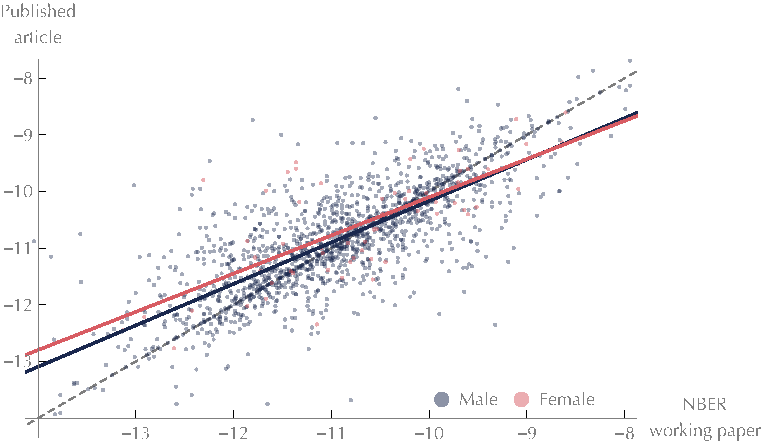
\includegraphics[width=12.3cm]{$HOME/Dropbox/Readability/draft/pdf/figure2.pdf}
		\floatfoot{\tiny \textit{Notes}. Sample 1,631 NBER working papers; 1,629 published articles. Data points represent each abstract's $-1\times\text{Dale-Chall}$ score pre-publicaction (NBER working paper) plotted against its $-1\times\text{Dale-Chall}$ post-publication score. Pink represents women co-authoring only with other women (65 NBER working papers; 64 published articles); blue are men co-authoring only with other men (1,566 NBER working papers; 1,565 published articles); articles co-authored by men and women are omitted. The line of best fit using OLS is shown separately for men and women. The grey dashed line is the 45 degree line through the origin; points above (below) it denote abstracts that were better written after (before) peer review.}
	}
\end{figure}